\documentclass{beamer}
%
% Choose how your presentation looks.
% For more themes, color themes and font themes, see:
% http://deic.uab.es/~iblanes/beamer_gallery/index_by_theme.html
%
\mode<presentation>
{
  \usetheme{Madrid}      % or try Darmstadt, Madrid, Warsaw, ...
  \usecolortheme{seahorse} % or try albatross, beaver, crane, ...
  \usefonttheme{serif}  % or try serif, structurebold, ...
  \setbeamertemplate{navigation symbols}{}
  \setbeamertemplate{caption}[numbered]
  \usepackage{amsmath}
  \usepackage{tcolorbox}
  \usepackage[export]{adjustbox}
  \tcbuselibrary{most}
  \usepackage{amsmath}  % conflicts with \oiint
  \usepackage{arydshln}
  \usepackage{tikz}
  \usetikzlibrary{plotmarks}
  \usepackage{pgfplots}
  \newcommand{\Ivec}[1]{\mbox{\boldmath $#1$}}
    \usepackage[normalem]{ulem}
    % \usepackage{tipa}
    \newcommand{\git}{\texttt{\textbf{git}}\xspace}
    \usepackage{listings}
} 


\definecolor{myblue}{RGB}{65,105,225} 
\definecolor{myorange}{RGB}{250,190,0}

\setbeamercolor{structure}{fg=white,bg=myorange}
\setbeamercolor*{palette primary}{fg=myblue,bg=myorange}
\setbeamercolor*{palette secondary}{fg=white,bg=myblue}
\setbeamercolor*{palette tertiary}{bg=myblue,fg=white}
\setbeamercolor*{palette quaternary}{fg=white,bg=myorange!50}

\setbeamercolor{frametitle}{fg=black!90!myblue}

\setbeamercolor{section in head/foot}{fg=white,bg=myblue}
\setbeamercolor{author in head/foot}{fg=black,bg=myorange}
\setbeamercolor{title in head/foot}{fg=white,bg=myblue}

\setbeamertemplate{navigation symbols}{}

\setbeamertemplate{itemize/enumerate body begin}{\large}
\setbeamertemplate{itemize/enumerate subbody begin}{\large}


\defbeamertemplate*{headline}{mytheme}
{%
  \begin{beamercolorbox}[ht=2.25ex,dp=3.75ex]{section in head/foot}
    \insertnavigation{\paperwidth}
  \end{beamercolorbox}%
}%

\defbeamertemplate*{footline}{mytheme}
{
  \leavevmode%
  \hbox{%
  \begin{beamercolorbox}[wd=.5\paperwidth,ht=2.25ex,dp=1ex,right]{author in head/foot}%
    \usebeamerfont{author in head/foot}\insertshortauthor\hspace*{2em}
  \end{beamercolorbox}%
  \begin{beamercolorbox}[wd=.5\paperwidth,ht=2.25ex,dp=1ex,left]{title in head/foot}%
    \usebeamerfont{title in head/foot}\hspace*{2em}\insertshortsubtitle\hspace*{2em}
    \insertframenumber{} / \inserttotalframenumber
  \end{beamercolorbox}}%
  \vskip0pt%
}

\usepackage[english]{babel}
\usepackage[utf8x]{inputenc}
\usepackage{xcolor}
\usepackage{listings}
\usepackage{pgf}  
\usepackage{textpos}
\usepackage{tabulary}
\usepackage{scrextend}
\usepackage{hyperref}
\usepackage{setspace}
\usepackage{rotating}
\lstset
{
    language=[LaTeX]TeX,
    breaklines=true,
    basicstyle=\tt\scriptsize,
    %commentstyle=\color{green}
    keywordstyle=\color{blue},
    %stringstyle=\color{black}
    identifierstyle=\color{magenta},
}
\newcommand{\bftt}[1]{\textbf{\texttt{#1}}}
%\newcommand{\comment}[1]{{\color[HTML]{008080}\textit{\textbf{\texttt{#1}}}}}
\newcommand{\cmd}[1]{{\color[HTML]{008000}\bftt{#1}}}
\newcommand{\bs}{\char`\\}
\newcommand{\cmdbs}[1]{\cmd{\bs#1}}
\newcommand{\lcb}{\char '173}
\newcommand{\rcb}{\char '175}
\newcommand{\cmdbegin}[1]{\cmdbs{begin\lcb}\bftt{#1}\cmd{\rcb}}
\newcommand{\cmdend}[1]{\cmdbs{end\lcb}\bftt{#1}\cmd{\rcb}}

\newcommand{\wllogo}{\textbf{Overleaf}}

\usepackage{hyperref}
\hypersetup{
    colorlinks=true,
    linkcolor=blue,
    filecolor=magenta,      
    urlcolor=cyan,
    pdftitle={Overleaf Example},
    pdfpagemode=FullScreen,
    }

\urlstyle{same}

% this is where the example source files are loaded from
% do not include a trailing slash
\newcommand{\fileuri}{https://raw.githubusercontent.com/GiancarloSucci/UniBo.IDSEPC.A2022/main/A2022.IDSEPCLaTeX/}

\newcommand{\perche}{perch\'{e}}
\newcommand{\affinche}{affinch\'{e}}
\newcommand{\se}{s\'{e}}
\newcommand{\a}{\`{a}}
\newcommand{\est}{\`{e}}

\usepackage{stackengine}
\def\Ruble{\stackengine{.67ex}{%
  \stackengine{.48ex}{\textsf{P}}{\rule{.8ex}{.12ex}\kern.6ex}{O}{r}{F}{F}{L}%
  }{\rule{.8ex}{.12ex}\kern.6ex}{O}{r}{F}{F}{L}\kern-.1ex}



%----------------------------------------------------------------------------------------
%	TITLE PAGE
%----------------------------------------------------------------------------------------
\title[L02]{Introduzione alla data science e al pensiero computazionale\\
Lezione 8: Revisione dei fondamenti di statistica} % The short title appears at the bottom of every slide, the full title is only on the title page

\author[{\tiny Giancarlo Succi }]{Giancarlo Succi\\\\ Dipartimento di Informatica -- Scienza e Ingegneria\\Universit\`{a} di Bologna\\
\bftt{g.succi@unibo.it}
} % Your name
\institute[unibo] % Your institution as it will appear on the bottom of every slide, may be shorthand to save space

\date{} % Date, can be changed to a custom date

\setbeamertemplate{navigation symbols}{}
\AtBeginSection[]
{
        \begin{frame}<beamer>{Outline}
                \tableofcontents[currentsection]
        \end{frame}
}

\begin{document}
\begin{frame}
\titlepage % Print the title page as the first slide

\end{frame}

%=============================================

\addtobeamertemplate{frametitle}{}{%
\begin{textblock*}{10mm}(-0.01mm,-0.95cm)

\includegraphics[width=0.9cm]{unibo-logo.png}
\end{textblock*}}

%=============================================


%---------------------------------------------
\begin{frame}
{\centerline{Probability -- History of the term}}
\begin{itemize}
\item Classical probability 
\item Frequency probability 
\item Axiomatic probability
\end{itemize}

\begin{center}
Evolution: Classical $\to$  Frequency  $\to$  Axiomatic
\end{center}
\end{frame}

%----------------------------------------------------------------------------------------

%------------------------------------------------

\begin{frame}
{\centerline{Classical probability. Definition }}
\Large{\textbf{Definition} If a random experiment (process with an uncertain outcome) can result in $n$ \textit{ mutually exclusive and equally likely} outcomes, and if $n_A$ of these outcomes has an attribute $A$, then the probability of $A$ is the fraction $n_A/n$.}

\end{frame}

%----------------------------------------------------------------------------------------

%------------------------------------------------

\begin{frame}
{\centerline{Classical probability. Definition }}

\Large{A basic assumption in the definition of classical probability is that $n$ is a finite number; that is, there is only a finite number of possible outcomes. If there is an infinite number of possible outcomes, the probability of an outcome is not defined \textbf{in the classical sense}.}

\end{frame}

%----------------------------------------------------------------------------------------

%------------------------------------------------

\begin{frame}
{\centerline{Classical probability. Examples }}
\begin{itemize}
\item Roll of a dice
\item Draw a card from a deck
\item Toss of a coin
\end{itemize}
%A basic assumption in the definition of classical probability is that 
\end{frame}

%----------------------------------------------------------------------------------------

\begin{frame}
{\centerline{Classical probability. Problems }}
\begin{itemize}
\item (Already mentioned) Infinite events\\
\item Definition of equally likely (circular)\\
\item Management of non physical problems for which there is no experiment
\end{itemize}
%A basic assumption in the definition of classical probability is that 
\end{frame}

%----------------------------------------------------------------------------------------


%------------------------------------------------

\begin{frame}
{\centerline{Frequency probability }}


\begin{itemize}
\item We start from considering the case of the outcomes not being equally likely and $n$ being potentially infinite.\\
\item In such cases, how might we define the probability of an outcome that has attribute ``a''?
\end{itemize}
 

\end{frame}

%----------------------------------------------------------------------------------------

%------------------------------------------------

\begin{frame}
{\centerline{Frequency probability }}
\textbf{Definition} We might take a random (finite) sample from the population of interest and identify the proportion of the sample with attribute ``a''. 
\newline

$$Freq_a = \frac{n_a}{n}$$
\newline

We \textbf{estimate} $Pr[a]$ with $Freq_a$.

\end{frame}

%----------------------------------------------------------------------------------------

%------------------------------------------------

\begin{frame}
{\centerline{Problems with frequency probability}}

\begin{itemize}
\item We cannot run infinite trials, and our stopping point may induce ambiguities or errors in results, e.g., tossing the coint $\ldots{}$ \\
\item What if we cannot run trials? This definition requires repeatable experiments.
\end{itemize}

\end{frame}

%----------------------------------------------------------------------------------------


%------------------------------------------------

\begin{frame}
{\centerline{Axiomatic probability -- Sample space}}
Definitions:
\begin{itemize}
\item The sample space $\Omega$ is the set of possible outcomes of an experiment.
\end{itemize}

For example:
\begin{itemize}
\item Tossing a coin, the sample space is \{ H, T \}
\item Tossing a coin twice, the sample space is \{ HH, HT, TH, TT \}
\item Rolling a dice, the sample space is \{1, 2, 3, 4, 5, 6\}
\item Football match, the sample space is \{W, L, D \}
\item Selecting a point in the interval (0,1), the sample space is S = (0,1)
\item Selecting a salary in the range [50K\Ruble, 200K\Ruble], the sample space is S = [50K\Ruble, 200K\Ruble]
\end{itemize}

\vspace*{0.5cm}
\textit{\small This and the following slides are inspired by: \url{https://faculty.math.illinois.edu/~kkirkpat/SampleSpace.pdf}}

\end{frame}

\begin{frame}
{\centerline{Axiomatic probability -- Events}}
Definitions:
\begin{itemize}
\item Subsets of $\Omega$ are called events. 
\end{itemize}

For example:
\begin{itemize}
\item Tossing a coin with the sample space  \{ H, T \}, an event E is \{ H \}
\item Tossing a coin twice with  sample space \{ HH, HT, TH, TT \}, an event E is \{ HH, TT \}
\item Rolling a dice with  sample space \{1, 2, 3, 4, 5, 6\}, an event E is  \{1, 3, 5 \}, \textit{the odd sides}
\item Football match with sample space  \{W, L, D \}, an event E is  \{W, D \}, \textit{not loosing}
\item Selecting a point in the interval (0,1) with the sample space S = (0,1), an event E is (0,1/2), \textit{the first half}
\item Selecting a salary in the range [50K\Ruble, 200K\Ruble], an event E is (150K\Ruble, 200K\Ruble], \textit{top salary}

\end{itemize}


\end{frame}


%----------------------------------------------------------------------------------------

%------------------------------------------------
\begin{frame}
{\centerline{Axiomatic probability -- Probability measure}}
A probability measure is a function $\mathbb{P}$ defined on the $\sigma$-algebra$^\dag$ of events $\mathcal{E}$ such that:
\begin{itemize}
\item $\forall A \in \mathcal{E}, \mathbb{P}(A) \geq 0$,
\item $\mathbb{P}(\Omega) = 1 $,
\item if $ A_1, A_2, \ldots \in \mathcal{E}$ are disjoint then 
$$\mathbb{P}\left( \bigcup_{i=1}^{\infty}A_i \right) = \sum_{i=1}^{\infty} \mathbb{P}(A_i).$$
\end{itemize}

\vspace*{1cm}
$^\dag$\textit{\small The definition of $\sigma$-algebra is omitted}

\end{frame}

%----------------------------------------------------------------------------------------

%------------------------------------------------
\begin{frame}
{\centerline{Axiomatic probability -- Probability space}}
The triple ($\Omega, \mathcal{E}, \mathbb{P}$) is called a \textbf{probability space}. 
\newline

For the example of rolling a dice:
\begin{itemize}
\item $\Omega$ - all possible outcomes: 1, 2, ... , 6
\item $\mathcal{E}$ - subsets of $\Omega$: 
\begin{itemize}
\item  \{1 \}
\item the odd sides:  \{1, 3, 5 \}
\item the small sides:  \{1, 2 \}
\item any side: \{1, 2, 3, 4, 5, 6\}
\end{itemize}
\item $\mathbb{P}$ - the probability measure of events from $\mathcal{E}$:
\begin{itemize}
\item $\mathbb{P}$(\{1\}) = 1/6
\item $\mathbb{P}$(the odd sides) = 1/2
\item $\mathbb{P}$(the small sides) = 1/3
\item $\mathbb{P}$(any side) = 1
\end{itemize}
\end{itemize}

\end{frame}

%----------------------------------------------------------------------------------------

\begin{frame}
{\centerline{Axiomatic probability -- Random variable}}

A \textbf{random variable} is a function $X : \Omega \to \mathbb{A}$ such that:
\begin{itemize}
\item $\mathbb{A}$ is a measurable space,
\item  for every real $a$, $\left\lbrace \omega \in \Omega: X(\omega) \leq a \right\rbrace \in \mathcal{E}$.
\end{itemize}

\vspace{0.5cm}
 Note that:
\begin{itemize}
\item Usually $\mathbb{A}$ is $\mathbb{R}$ or a subset of it
\item A random variable is NOT a variable but a function
\end{itemize}

\end{frame}
%------------------------------------------------
\begin{frame}
{\centerline{Example of random variable (1/2)}}

Tossing a dice three times:
\begin{itemize}
\item the sample space $\Omega$ is \{ 111, 112, 113, 211, $\ldots{}$ \}
\item events E$_i$ are:
\begin{itemize}
\item \{ 222 \}
\item \{ 111, 555 \}
\item \{ 123, 456, 531 \}
\item $\ldots{}$
\end{itemize}
\item the probability measure is the function $\mathbb{P}$
\begin{itemize}
\item $\mathbb{P}$(\{ 222 \}) = 1/216
\item $\mathbb{P}$(\{ 111, 555 \}) = 1/108
\item $\mathbb{P}$(\{ 123, 456, 531 \}) = 1/72
\item $\mathbb{P}$($\ldots{}$)
\item $\ldots{}$
\end{itemize}

\end{itemize}

\end{frame}

\begin{frame}
{\centerline{Example of random variable (2/2)}}

Tossing a dice three times:
\begin{itemize}
\item a random variable $X$ is the sum of the three results
\item the sample space $\Omega_X$ is \{ 3, 4, 5, 6, 7, 8, 9, $\ldots{}$ , 18\}
\item events E$_{X,i}$ are: 
\begin{itemize}
\item \{ 3\} 
\item \{4, 6 \} 
\item \{ 16, 17, 18 \}
\item $\ldots{}$
\end{itemize}
\item the probability measure is the function $\mathbb{P}_{X}$
\begin{itemize}
\item $\mathbb{P}_{X}$( \{ 3\} ) = 1/216
\item  $\mathbb{P}_{X}$(\{4, 6 \}) = 13/216
\item  $\mathbb{P}_{X}$(\{ 16, 17, 18 \}) = 10 / 216 = 5/108
\item $\ldots{}$
\end{itemize}
\end{itemize}


\end{frame}



%----------------------------------------------------------------------------------------

\begin{frame}
{\centerline{Axiomatic probability -- Pdf}}
Given:
\begin{itemize}
\item A random variable $X$
\item A set in which it is defined $S$ (called the support)
\item A \textbf{probability density function} (pdf) is a function $f(X) \geq 0, X \in S$
\item defined for the continuous case as:
$$\mathbb{P}(S) = \int_S f(X)dX $$
\end{itemize}

\end{frame}

%-------------

\begin{frame}
{\centerline{Axiomatic probability -- Pdf -- Example }}
Example: Uniform distribution:

pdf:
\begin{center}
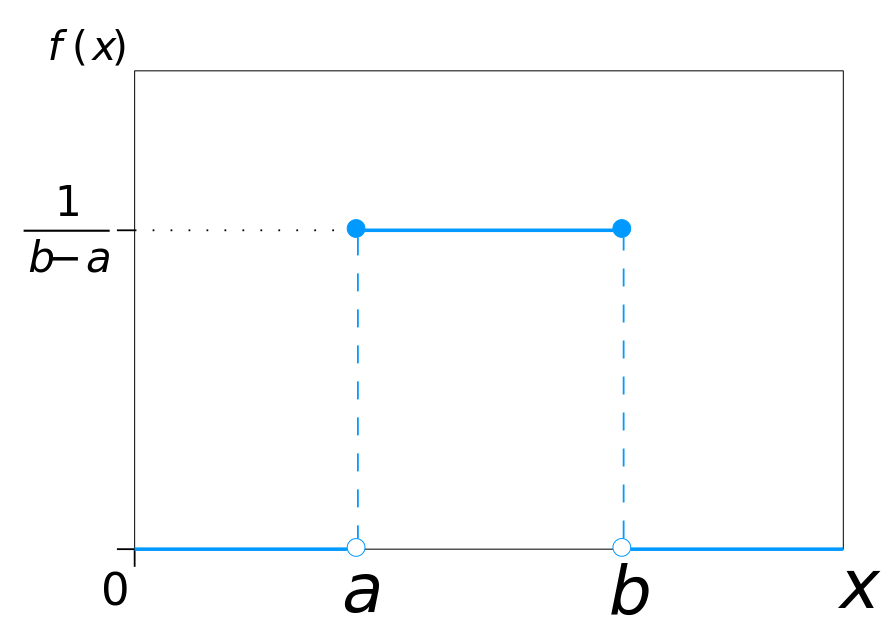
\includegraphics[width=8cm]{A2022.FondamentiStatistica/Uniform_Distribution_PDF_SVG_svg.png}
\end{center} 
% CDF:
% \begin{center}
% 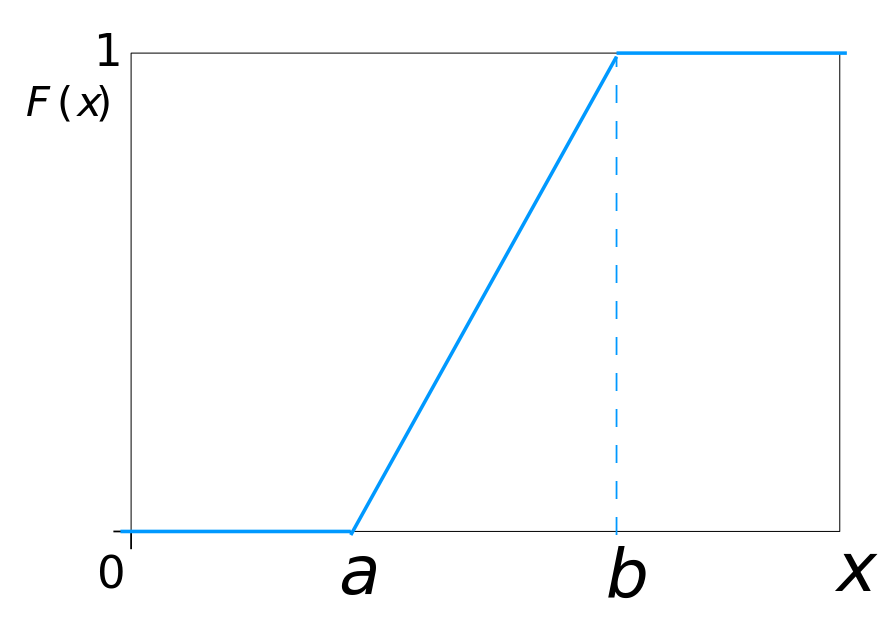
\includegraphics[width=4cm]{A2022.FondamentiStatistica/Uniform_cdf_svg.png}
% \end{center}

\end{frame}

%-------------

%----------------------------------------------------------------------------------------

\begin{frame}
{\centerline{Axiomatic probability -- Pmf}}
Given:
\begin{itemize}
\item A random variable $X$
\item A set in which it is defined $S$ (called the support again)
\item A \textbf{probability mass function} (pdf) is a function $f(X) \geq 0, X \in S$
\item defined for the discrete case as:
$$\mathbb{P}(S) = \sum_{S} f(X) $$
\end{itemize}

\end{frame}

%-------------


\begin{frame}
{\centerline{Axiomatic probability -- Pmf -- Example 1}}
Example 1: Discrete Uniform distribution:

pmf:
\begin{center}
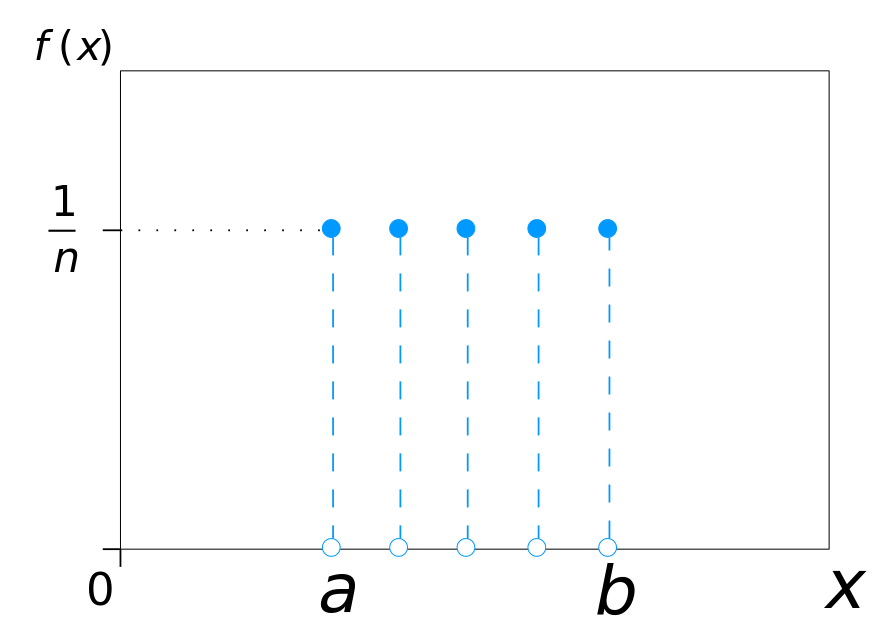
\includegraphics[width=8cm]{A2022.FondamentiStatistica/Uniform_discrete_pmf_svg_svg.png}
\end{center} 
% CDF:
% \begin{center}
% 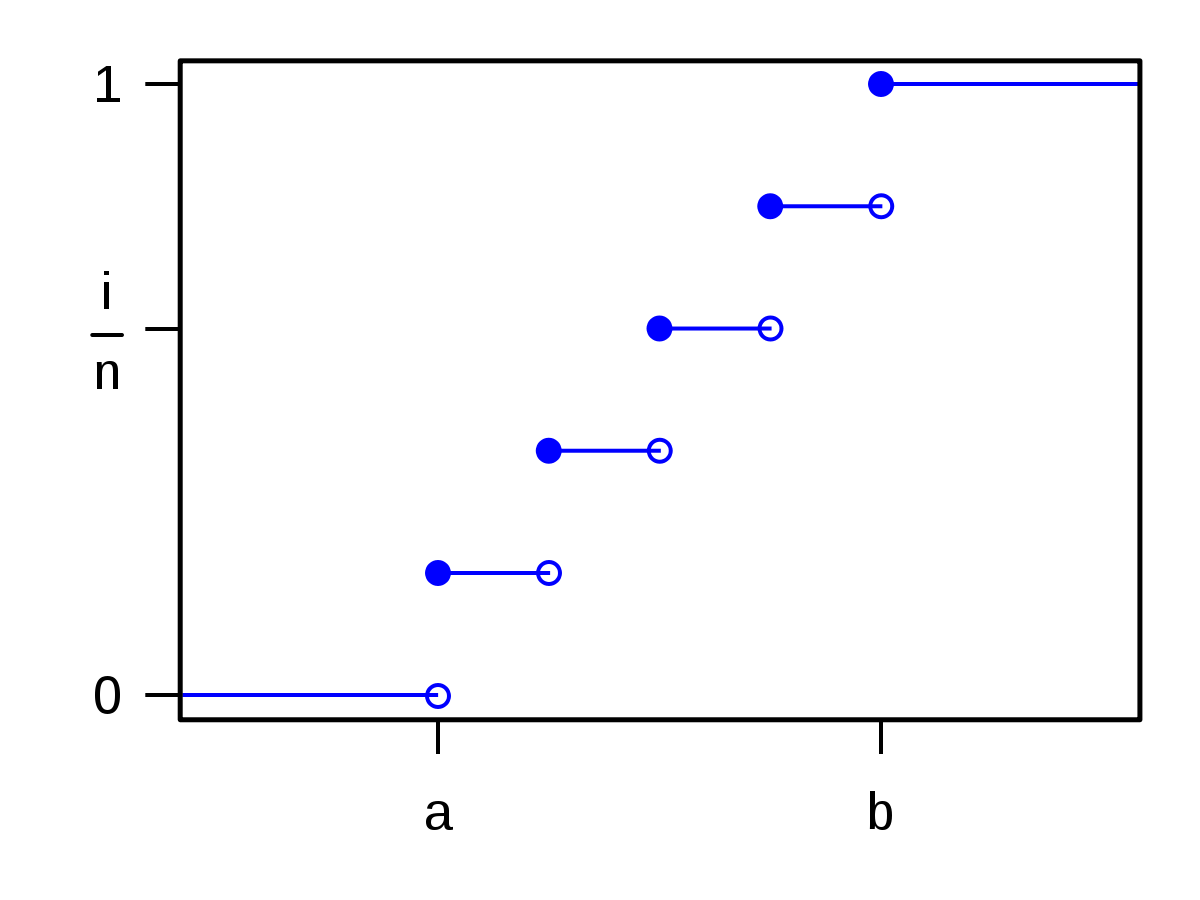
\includegraphics[width=4cm]{A2022.FondamentiStatistica/1200px-Dis_Uniform_distribution_CDF_svg.png}
% \end{center}

\end{frame}
%------------------------------------------------

\begin{frame}
{\centerline{Axiomatic probability -- Pmf -- Example 2}}
Example 2: Computing the score of rolling a dice three times:

pmf:
\begin{center}
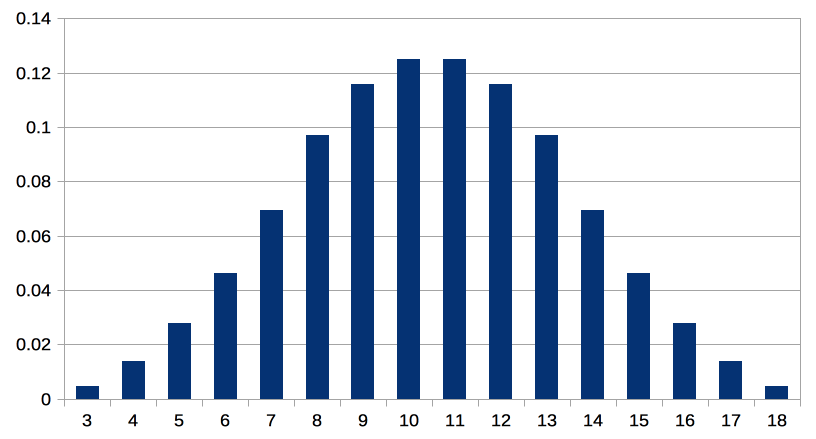
\includegraphics[width=8cm]{A2022.FondamentiStatistica/RollingADiceThreeTimes.png}
\end{center} 

\end{frame}
%------------------------------------------------

\begin{frame}
{\centerline{Axiomatic probability -- Cdf (continuous)}}
Given:
\begin{itemize}
\item A random variable $X$
\item A set in which it is defined $S$ (called the support)
\item The probability density function of $X$, $f_X$
\item We define the \textbf{(cumulative) distribution function} of $X$ in the continuous case as:
$$F_X(x) = \mathbb{P}(X \leq x) =  \int_{-\infty}^{x} f_X(w)dw $$

\end{itemize}

\vspace*{1cm}
\textit{Note. The subscript $X$ is sometimes omitted, so we often write $F$ instead of $F_X$.}
\end{frame}



%----------------------------------------------------------------------------------------

\begin{frame}
{\centerline{Axiomatic probability -- Cdf -- Example}}
Example: Uniform distribution:

cdf:
\begin{center}
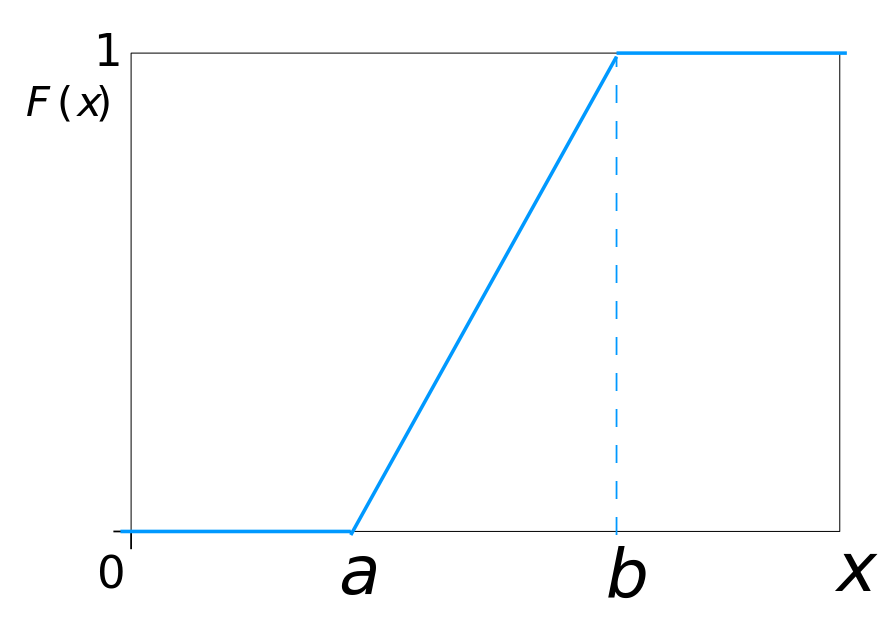
\includegraphics[width=8cm]{A2022.FondamentiStatistica/Uniform_cdf_svg.png}
\end{center}

\end{frame}

%----------------------------------------------------------------------------------------



\begin{frame}
{\centerline{Axiomatic probability -- Cdf (discrete)}}
Given:
\begin{itemize}
\item A random variable $X$
\item A set in which it is defined $S$ (called the support)
\item The probability mass function of $X$, $f_X$
\item We define the \textbf{(cumulative) distribution function} of $X$ in the discrete case as:
$$F_X(x) = \mathbb{P}(X \leq x) =  \sum_{w\leq x} f_X(w)$$
\end{itemize}

\vspace*{1cm}
\textit{Note. The subscript $X$ is sometimes omitted, so we often write $F$ instead of $F_X$.}

\end{frame}

%----------------------------------------------------------------------------------------

\begin{frame}
{\centerline{Axiomatic probability -- Cdf -- Example 1}}
Example 1: Discrete uniform distribution:


cdf:
\begin{center}
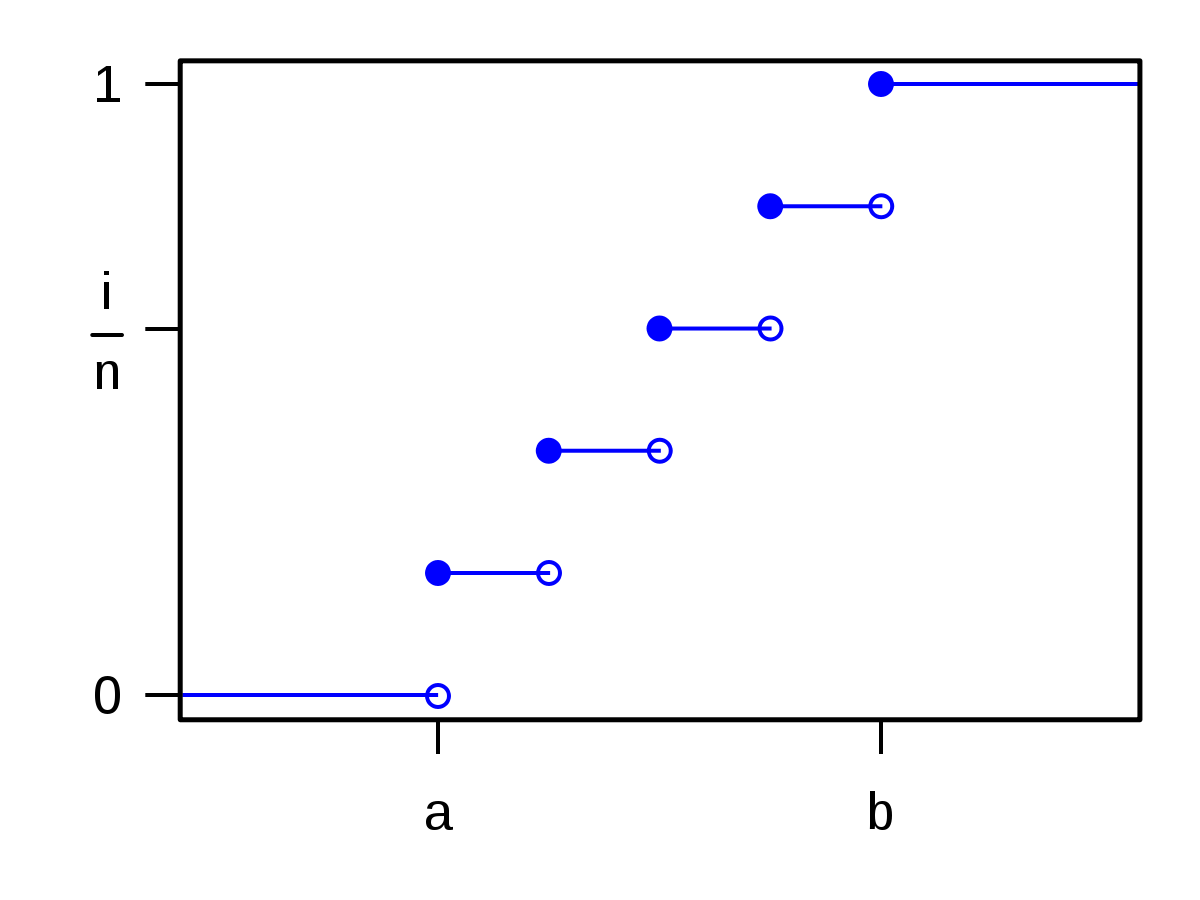
\includegraphics[width=8cm]{A2022.FondamentiStatistica/1200px-Dis_Uniform_distribution_CDF_svg.png}
\end{center}

\end{frame}
%------------------------------------------------

\begin{frame}
{\centerline{Axiomatic probability -- Cdf -- Example 2}}
Example 2: Computing the score of rolling a dice three times:

cmf:
\begin{center}
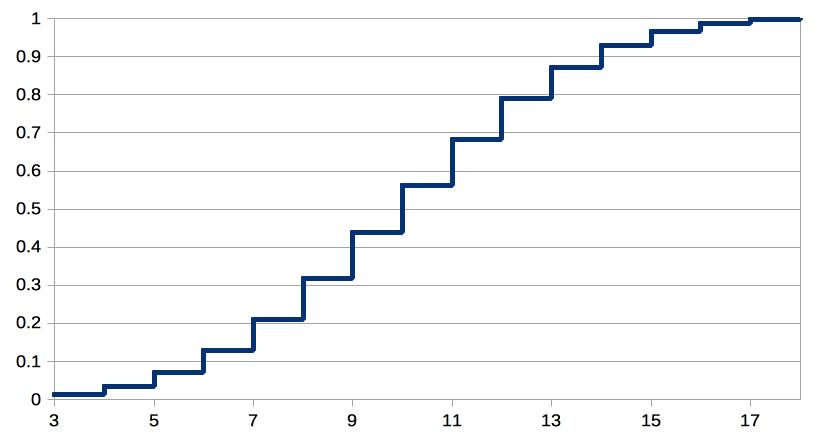
\includegraphics[width=8cm]{A2022.FondamentiStatistica/RollingADiceThreeTimes_cdf.png}
\end{center} 

\end{frame}
%------------------------------------------------

%------------------------------------------------
\begin{frame}
{\centerline{Axiomatic probability -- Expected value}}

Let:
\begin{itemize}
\item $x$ be a random variable
\item $a(x)$ be a function of $x$
\item $F$ be its cdf
\item $f$ be its pdf or pmf (if discrete)
\end{itemize}

The \textbf{expected value} of $a(X)$ is:

\begin{itemize}
\item In continuous:
 $$\mathbb{E}(a(X)) = \int_{x \in S} a(x)f(x)dx$$
\item In discrete: 
 $$\mathbb{E}(a(X)) = \sum_{j} a(x_j)f(x_j)$$
\end{itemize}


\end{frame}
%----------------------------------------------------------------------------------------

%------------------------------------------------
\begin{frame}
{\centerline{Basic definitions -- Mean (continuous)}}


Let $ a(X) = X$, then the mean of $X$ is: \\
\begin{itemize}
\item in the continuous case: $$\mu = \mathbb{E}(X) = \int_{x \in S} xf(x)dx $$
\end{itemize}
where S is the Support.

\end{frame}


%------------------------------------------------
\begin{frame}
{\centerline{Example of mean (continuous)}}


Example: Uniform distribution on an interval [a,b]. 

pdf = $\frac{1}{b-a}$ if $x \in [a,b]$ and pdf=0 elsewhere

Mean: $$\mu = \mathbb{E}(X) = \int_{-\infty}^{+\infty} x \frac{1}{b-a} dx  = \frac{1}{b-a} \left(\frac{x^2}{2}\right)\bigg|_a^b =$$ $$= \frac{1}{2} * \frac{1}{b-a} * (b^2 - a^2) = \frac{1}{2} (a+b) $$ 

%\textcolor{red}{\bf(add examples)}\\

%\textcolor{blue}{\bf(please from now on, try to replicate my corrections in the remaining slides)}


\end{frame}


%------------------------------------------------
\begin{frame}
{\centerline{Basic definitions -- Mean (discrete)}}


Let $ a(X) = X$, then the mean of $X$ is: \\
\begin{itemize}
\item in discrete case: $$\mu = \mathbb{E}(X) = \sum_{j} x_jf(x_j) $$
\end{itemize}


\end{frame}

%------------------------------------------------

%------------------------------------------------
\begin{frame}
{\centerline{Example of mean (discrete)}}



Example: a dice with 6 edges (6 outcomes: $X=$ \{1, 2, 3, 4, 5, 6\}). PMF equals 1/6 for each outcome.

Mean: $$\mu = \mathbb{E}(X) = \sum_{x \in X} x \frac{1}{6} =  $$

$$=1*\frac{1}{6} + 2*\frac{1}{6} + 3*\frac{1}{6} + 4*\frac{1}{6} + 5*\frac{1}{6} + 6*\frac{1}{6} = $$ 
$$= \frac{1}{6} (1+2+3+4+5+6) = 3.5$$

\end{frame}

%------------------------------------------------



%------------------------------------------------

\begin{frame}
{\centerline{Basic definitions -- Variance}}

\textbf{Variance} of random variable:
$$\mathbb{V}(X)=\mathbb{E}[(X-\mathbb{E}(X))^2]$$

\begin{itemize}
\item for discrete case: $\mathbb{V}(X)= \sum_{j} (x_j-\mu)^2 f(x_j)$
\item for continuous case: $\mathbb{V}(X)= \int\displaylimits_{S} (x -\mu)^2 f(x) dx$
\end{itemize}
\end{frame}


%------------------------------------------------

\begin{frame}
{\centerline{Example of variance}}

Example: Uniform distribution on an interval [a,b]. $\mu = \frac{1}{2}(a+b)$

$$\mathbb{V}(X)= \int\displaylimits_{-\infty}^{+\infty} (x -\mu)^2 \frac{1}{b-a} dx = $$
$$ = \int\displaylimits_{-\infty}^{+\infty} (x -\frac{1}{2} (a+b))^2 \frac{1}{b-a} dx =
\frac{1}{b-a} \left(\frac{(x-\frac{1}{2} (a+b))^3}{3}\right)\bigg|_a^b =$$
$$ = \frac{1}{3\cdot 2^3 (b-a)} ((b-a)^3-(a-b)^3) = \frac{1}{12}(b-a)^2$$
\end{frame}

%------------------------------------------------

\begin{frame}
{\centerline{Basic definitions -- $\alpha$-quantile}}

\textbf{$\alpha$-quantile} ($\alpha \in (0,1)$):
$$X_\alpha: \mathbb{P}(X \leq X_\alpha) = \alpha;$$
$$\mathbb{P}(X > X_\alpha) = 1 - \alpha.$$


\end{frame}

%------------------------------------------------
\begin{frame}
{\centerline{Basic definitions -- Median}}



Median (\textbf{$0.5$-quantile}):
$$X_{0.5}: \mathbb{P}(X \leq X_{0.5}) = 0.5;$$
$$\mathbb{P}(X > X_{0.5}) = 0.5$$

% \textcolor{red}{\bf(add an example)}
\end{frame}


%------------------------------------------------
\begin{frame}
{\centerline{Basic definitions -- Mode}}

Mode (the most frequent element):
$$mode = argmax(f(x))$$ 

% \textcolor{red}{\bf(add an example)}

\end{frame}


%----------------------------------------------------------------------------------------

%------------------------------------------------
\begin{frame}
{\centerline{Mean. Median. Mode. Examples}}
\begin{center}
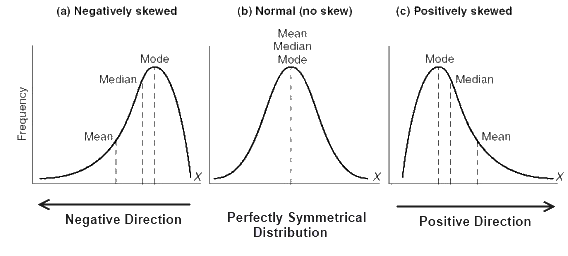
\includegraphics[width=12cm]{A2022.FondamentiStatistica/mode3.png}
\end{center} 
\end{frame}


%----------------------------------------------------------------------------------------

%------------------------------------------------
\begin{frame}
{\centerline{Normal distribution}}
% \textbf{with parameters $\mu, \sigma $}

The random variable X has a \textbf{normal distribution} with mean $\mu$ and variance $\sigma^2$ if it has density:
$$\phi(x) = \frac{1}{\sqrt[]{2\pi\sigma^2}} e^{-\frac{(x-\mu)^2}{2\sigma^2}}; $$
and CDF: 
$$\Phi(x) = \frac{1}{\sqrt[]{2\pi\sigma^2}} \int_{-\infty}^{x} e^{-\frac{(t-\mu)^2}{2\sigma^2}} dt.$$

We write $X \sim N(\mu,\sigma^2).$
\end{frame}

%----------------------------------------------------------------------------------------

%------------------------------------------------
\begin{frame}
{\centerline{Standard Normal distribution}}

The random variable Z has a \textbf{standard normal distribution} if $\mu=0$ and $\sigma=1$. Hence it has density:
$$\phi(z) = \frac{1}{\sqrt[]{2\pi}} e^{-z^2/2}; $$
and CDF: 
$$\Phi(x) = \frac{1}{\sqrt[]{2\pi}} \int_{-\infty}^{x} e^{-t^2/2} dt.$$

We write $Z \sim N(0,1).$ 

The $\alpha$ upper quantile is denoted by $z_\alpha$. Thus, if $Z \sim N(0,1)$, then we write $\mathbb{P}(Z>z_\alpha) = \alpha.$

\end{frame}



%----------------------------------------------------------------------------------------

%------------------------------------------------
\begin{frame}
{\centerline{Normal distribution}}
$$X \in \mathbb{R} \sim N(\mu,\sigma^2), \sigma^2 > 0$$
$$F(x) = \Phi(\frac{x-\mu}{\sigma})$$
$$f(x) = \frac{1}{\sigma}\phi(\frac{x-\mu}{\sigma})$$
%$$\phi(z) = \frac{1}{\sqrt[]{2\pi}} e^{-z^2/2}; $$
%$$\Phi(x) = \frac{1}{\sqrt[]{2\pi}} \int_{-\infty}^{x} e^{-t^2/2} dt.$$


\begin{center}
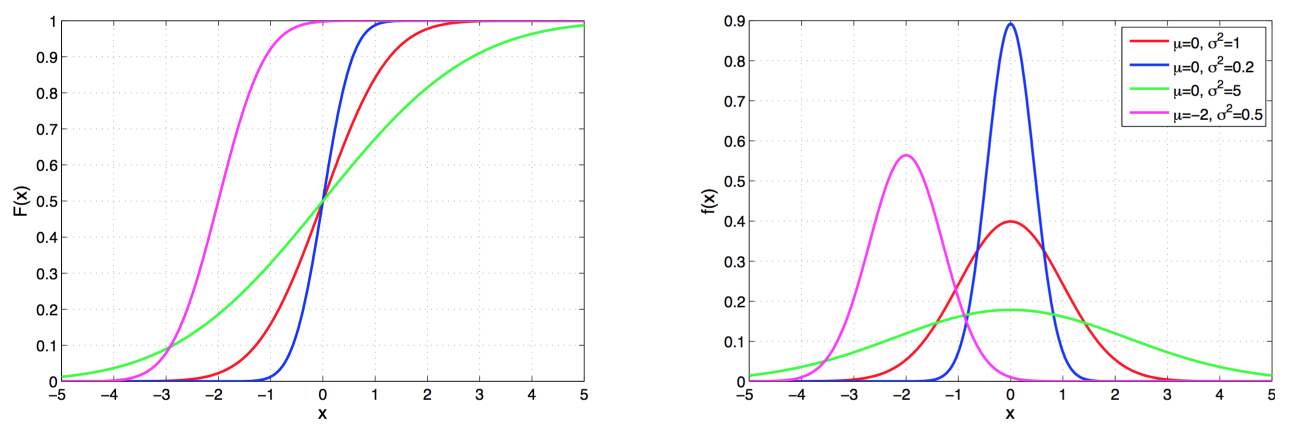
\includegraphics[width=11.5cm]{A2022.FondamentiStatistica/norm-distr.jpg}
\end{center} 
\end{frame}

\begin{frame}
{\centerline{Exercise 1}}
\begin{itemize}
    \item A discrete random variable has the following probability mass function defined as:
    \newline
    \begin{center}
        \resizebox{0,5\textwidth}{!}{%
  \begin{tabular}{|c|c|c|c|c|}
  \hline
  $x$ & 0 &2&4&6\\
  \hline
  $P(X=x)$ & $\frac{1}{7}$  & $\frac{3}{7}$  & $\frac{1}{7}$  & $\frac{2}{7}$\\
  \hline
  \end{tabular}
} % end of scope of "\resizebox"  directive

    \end{center}

    \newline
    \item Compute:
    \begin{itemize}
        \item mean
        \item median
        \item mode
        \item variance
        \item standard deviation
    \end{itemize}
\end{itemize}
\end{frame}

\begin{frame}
{\centerline{Exercise 1 -- solution}}
\begin{itemize}
    \item A discrete random variable has the following probability mass function defined as:
    \newline
    \begin{center}
        \resizebox{0,9\textwidth}{!}{%
  \begin{tabular}{|c|c|c|c|c|}
  \hline
  $x$ & 0 &2&4&6\\
  \hline
  $P(X=x)$ & $\frac{1}{7}$  & $\frac{3}{7}$  & $\frac{1}{7}$  & $\frac{2}{7}$ \\
  \hline
   $x \times P(X=x)$ & $0$  & $0,857$  & $0,571$  & $1,714$ \\
   \hline
   $x - \overline{x}$ & $-3,143$  & $-1,143$  & $0,857$  & $2,857$ \\
   \hline
   $(x - \overline{x})^{2}$ & $9,878$  & $1,306$  & $0,735$  & $8,163$ \\
   \hline
   $(x - \overline{x})^{2} \times P(X=x)$ & $1,411$  & $0,560$  & $0,105$  & $2,332$ \\
   \hline

  \end{tabular}
} % end of scope of "\resizebox"  directive

    \end{center}
    \newline
    
    \item So we get:
    \begin{itemize}
        \item $ \overline{x} = \sum (x \times P(X=x)) = 3,143 $
        \item $ \mathbb{V}(x) = \sum ((x - \overline{x})^{2} \times P(X=x)) = 4,408 $

    \end{itemize}

\end{itemize}
\end{frame}

\begin{frame}
{\centerline{Exercise 2}}
\begin{itemize}
    \item A discrete random variable has the following probability mass function defined as:
    \newline
    \begin{center}
        \resizebox{0,5\textwidth}{!}{%
  \begin{tabular}{|c|c|c|c|c|c|}
  \hline
  $x$ & 1 &2&3&4&5\\
  \hline
  $P(X=x)$ & $\frac{2}{10}$  & $\frac{2}{10}$  & $k$  & $\frac{3}{10}$\frac{1}{10}\\
  \hline
  \end{tabular}
} % end of scope of "\resizebox"  directive

    \end{center}

    \newline
    \item Compute:
    \begin{itemize}
        \item the value of k
        \item mean
        \item median
        \item mode
        \item variance
        \item standard deviation
    \end{itemize}
\end{itemize}
\end{frame}


\begin{frame}
{\centerline{Exercise 3}}
\begin{itemize}
    \item A continuous random variable X has probability density function defined as:
    \begin{equation*}
        
  f(x)=\left\{
        \begin{array}{ll}
             \frac{x^{2}}{9}, & \mbox{if $0<x<3$}\\
                0, & \mbox{elsewhere}
         \end{array}
        \right.
    \end{equation*}
    \newline
    \item Compute:
    \begin{itemize}
        \item mean
        \item median
        \item mode
        \item variance
        \item standard deviation
    \end{itemize}
\end{itemize}
\end{frame}

\begin{frame}
{\centerline{Exercise 3 -- solution}}
\begin{itemize}
    \item A continuous random variable X has probability density function defined as:
    \begin{equation*}
        
  f(x)=\left\{
        \begin{array}{ll}
             \frac{x^{2}}{9}, & \mbox{if $0<x<3$}\\
                0, & \mbox{elsewhere}
         \end{array}
        \right.
    \end{equation*}
    \newline
    \item Compute:
    \begin{itemize}
        \item mean = 2,25
        \item median $\approx$ 2,38
        \item mode = 3
        \item variance = 0,3375
        \item standard deviation = 0,581
    \end{itemize}
\end{itemize}
\end{frame}

\begin{frame}
{\centerline{Exercise 4}}
\begin{itemize}
    \item A continuous random variable X has probability density function defined as:
    \begin{equation*}
        
  f(x)=\left\{
        \begin{array}{ll}
             \frac{\sin(x)}{2}, & \mbox{if $0 \leq x \leq \pi$}\\
                0, & \mbox{elsewhere}
         \end{array}
        \right.
    \end{equation*}
    \newline
    \item Compute:
    \begin{itemize}
        \item mean
        \item median
        \item mode
        \item variance
        \item standard deviation
    \end{itemize}
\end{itemize}
\end{frame}

\begin{frame}
{\centerline{Exercise 4 - solution}}
\begin{itemize}
    \item A continuous random variable X has probability density function defined as:
    \begin{equation*}
        
  f(x)=\left\{
        \begin{array}{ll}
             \frac{\sin(x)}{2}, & \mbox{if $0 \leq x \leq \pi$}\\
                0, & \mbox{elsewhere}
         \end{array}
        \right.
    \end{equation*}
    \newline
    \item Compute:
    \begin{itemize}
        \item mean = $\frac{\pi}{2}$
        \item median = $\frac{\pi}{2}$
        \item mode = $\frac{\pi}{2}$
        \item variance  = $\frac{\pi^{2}}{4}$ - 2 $\approx$ 0,467
        \item standard deviation $\approx$ 0,684
    \end{itemize}
\end{itemize}
\end{frame}


\begin{frame}
{\centerline{Domande?}}
\vspace{1cm}
\begin{center}
    \LARGE{Fine della lezione otto.}
\end{center}

\end{frame}


\end{document}
